\documentclass{standalone}
\usepackage{tikz}
\usetikzlibrary{patterns, positioning}
\usepackage[sfdefault]{ClearSans} %% option 'sfdefault' activates Clear Sans as the default text font
\usepackage[T1]{fontenc}

\begin{document}
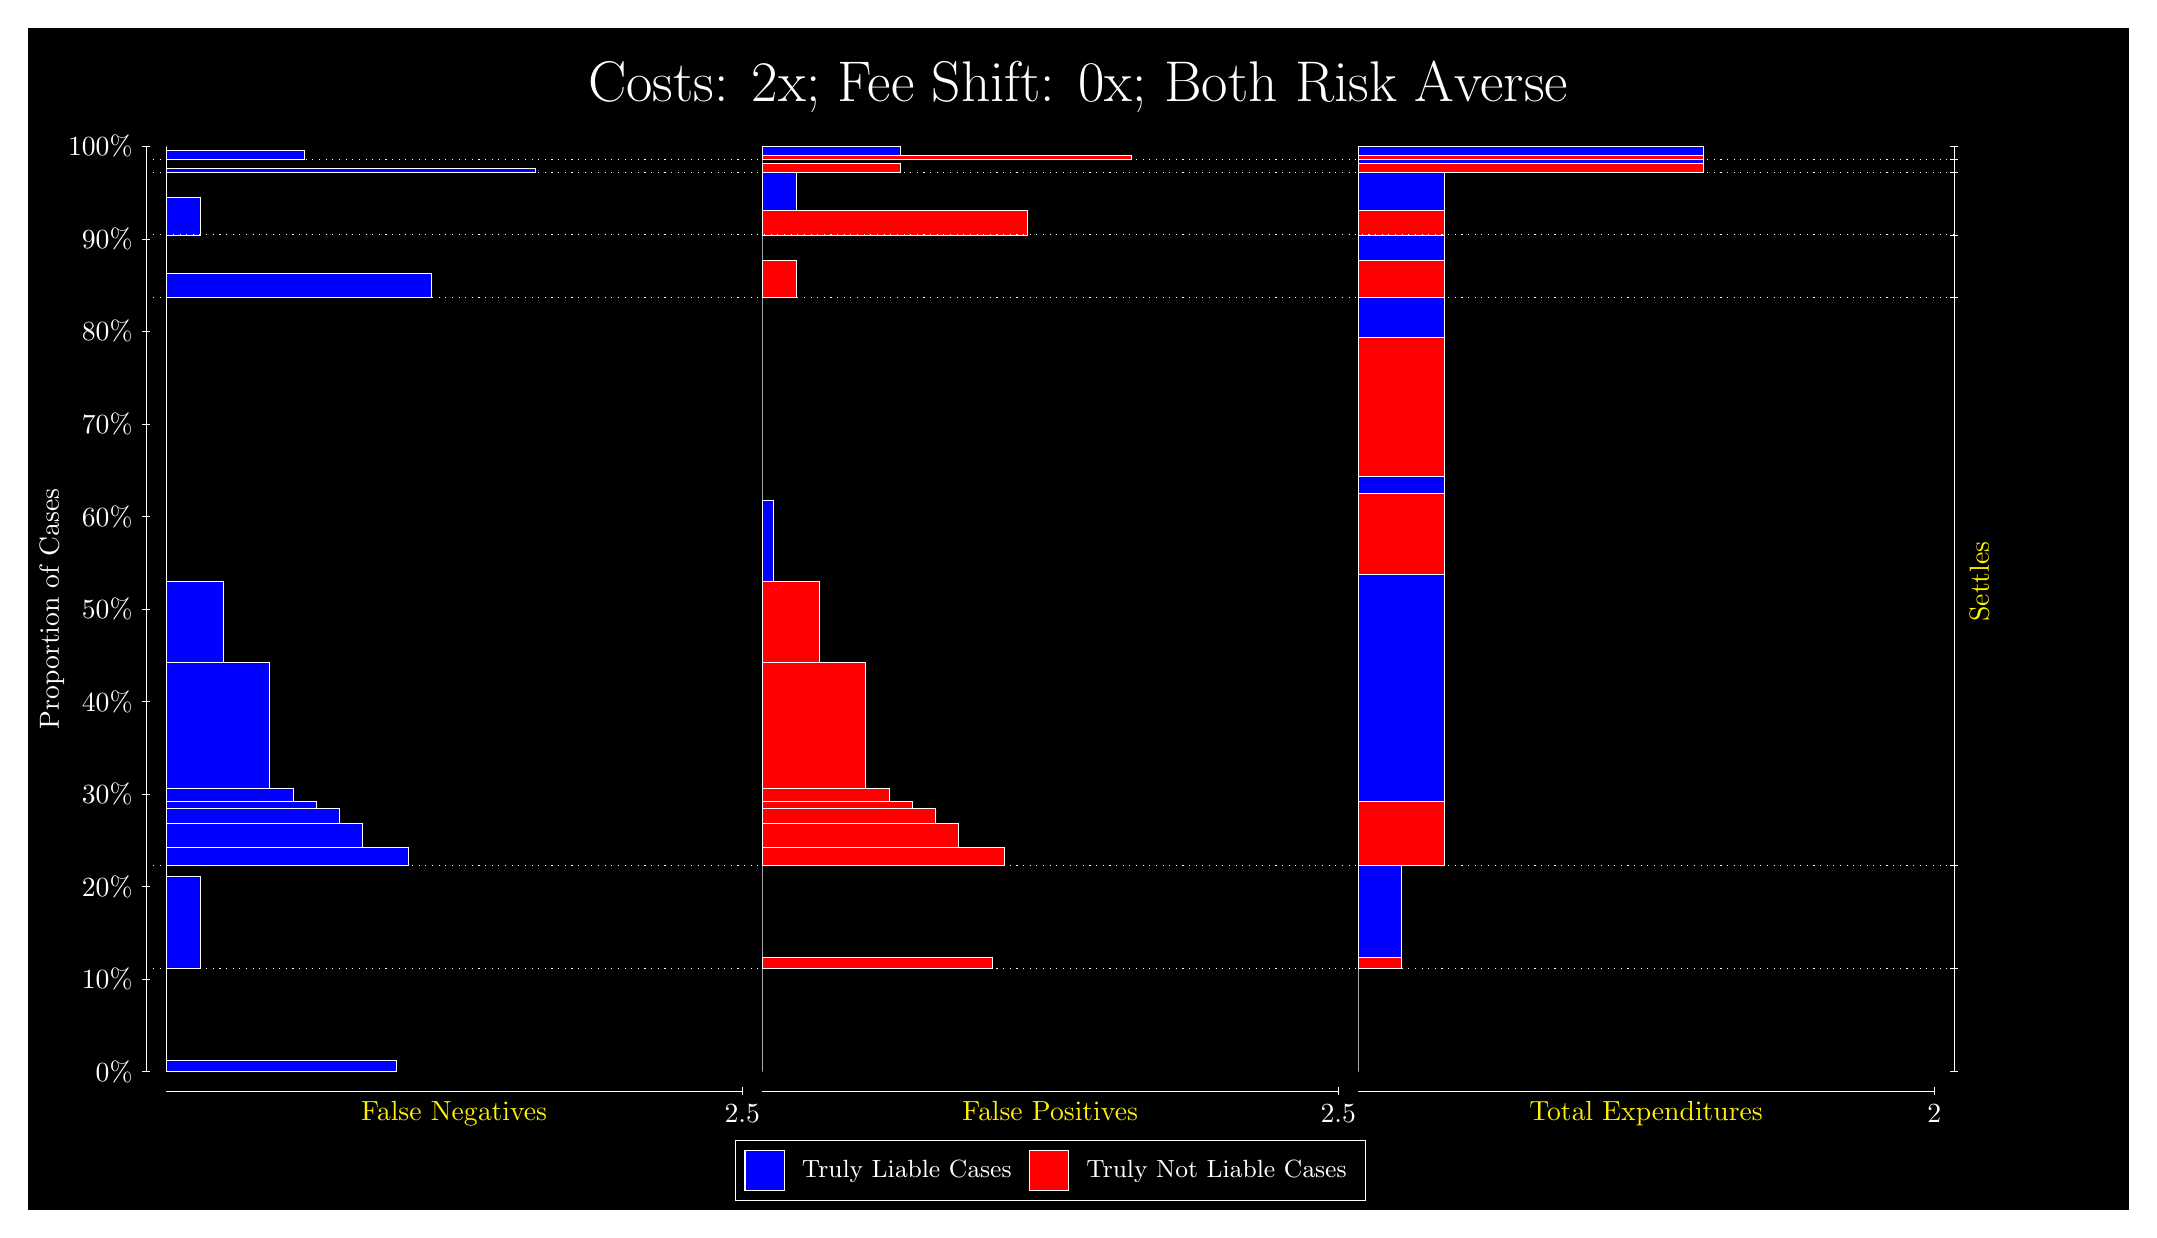
\begin{tikzpicture}
\draw[fill=black] (0,0) rectangle (26.667,15);
\draw[text=white] (0,13.5) rectangle (26.667,15) node[midway] {\huge Costs: 2x; Fee Shift: 0x; Both Risk Averse};
\draw[white, very thin] (1.5,1.75) -- (1.5,13.5);
\node[rotate=90, text=white, anchor=center] at (0.3, 7.625) {Proportion of Cases};
\draw[white, very thin] (1.45,1.75) -- (1.55,1.75);
\node[text=white, anchor=east] at (1.45, 1.75) {0\%};
\draw[white, very thin] (1.45,2.925) -- (1.55,2.925);
\node[text=white, anchor=east] at (1.45, 2.925) {10\%};
\draw[white, very thin] (1.45,4.1) -- (1.55,4.1);
\node[text=white, anchor=east] at (1.45, 4.1) {20\%};
\draw[white, very thin] (1.45,5.275) -- (1.55,5.275);
\node[text=white, anchor=east] at (1.45, 5.275) {30\%};
\draw[white, very thin] (1.45,6.45) -- (1.55,6.45);
\node[text=white, anchor=east] at (1.45, 6.45) {40\%};
\draw[white, very thin] (1.45,7.625) -- (1.55,7.625);
\node[text=white, anchor=east] at (1.45, 7.625) {50\%};
\draw[white, very thin] (1.45,8.8) -- (1.55,8.8);
\node[text=white, anchor=east] at (1.45, 8.8) {60\%};
\draw[white, very thin] (1.45,9.975) -- (1.55,9.975);
\node[text=white, anchor=east] at (1.45, 9.975) {70\%};
\draw[white, very thin] (1.45,11.15) -- (1.55,11.15);
\node[text=white, anchor=east] at (1.45, 11.15) {80\%};
\draw[white, very thin] (1.45,12.325) -- (1.55,12.325);
\node[text=white, anchor=east] at (1.45, 12.325) {90\%};
\draw[white, very thin] (1.45,13.5) -- (1.55,13.5);
\node[text=white, anchor=east] at (1.45, 13.5) {100\%};

\draw[white, very thin] (24.457,1.75) -- (24.457,13.5);
\draw[white, very thin] (24.407,1.75) -- (24.507,1.75);
\node[anchor=west] at (24.407, 1.75) {};
\draw[white, very thin] (24.407,3.0618) -- (24.507,3.0618);
\node[anchor=west] at (24.407, 3.0618) {};
\draw[white, very thin] (24.407,4.3703) -- (24.507,4.3703);
\node[anchor=west] at (24.407, 4.3703) {};
\draw[white, very thin] (24.407,11.579) -- (24.507,11.579);
\node[anchor=west] at (24.407, 11.579) {};
\draw[white, very thin] (24.407,12.375) -- (24.507,12.375);
\node[anchor=west] at (24.407, 12.375) {};
\draw[white, very thin] (24.407,13.171) -- (24.507,13.171);
\node[anchor=west] at (24.407, 13.171) {};
\draw[white, very thin] (24.407,13.335) -- (24.507,13.335);
\node[anchor=west] at (24.407, 13.335) {};
\draw[white, very thin] (24.407,13.5) -- (24.507,13.5);
\node[anchor=west] at (24.407, 13.5) {};

\draw[white, very thin, fill=blue] (1.75,1.75) rectangle (4.6775,1.888);
\draw[white, very thin, fill=red] (1.75,1.888) rectangle (1.75,3.0618);
\draw[white, very thin, fill=blue] (1.75,3.0618) rectangle (2.1891,4.2339);
\draw[white, very thin, fill=red] (1.75,4.2339) rectangle (1.75,4.3703);
\draw[white, very thin, fill=blue] (1.75,4.3703) rectangle (4.8239,4.5936);
\draw[white, very thin, fill=blue] (1.75,4.5936) rectangle (4.2384,4.9059);
\draw[white, very thin, fill=blue] (1.75,4.9059) rectangle (3.9457,5.0994);
\draw[white, very thin, fill=blue] (1.75,5.0994) rectangle (3.6529,5.1884);
\draw[white, very thin, fill=blue] (1.75,5.1884) rectangle (3.3602,5.3512);
\draw[white, very thin, fill=blue] (1.75,5.3512) rectangle (3.0674,6.9488);
\draw[white, very thin, fill=blue] (1.75,6.9488) rectangle (2.4819,7.9744);
\draw[white, very thin, fill=red] (1.75,7.9744) rectangle (1.75,11.579);
\draw[white, very thin, fill=blue] (1.75,11.579) rectangle (5.1167,11.894);
\draw[white, very thin, fill=red] (1.75,11.894) rectangle (1.75,12.375);
\draw[white, very thin, fill=blue] (1.75,12.375) rectangle (2.1891,12.856);
\draw[white, very thin, fill=red] (1.75,12.856) rectangle (1.75,13.171);
\draw[white, very thin, fill=blue] (1.75,13.171) rectangle (6.4341,13.218);
\draw[white, very thin, fill=red] (1.75,13.218) rectangle (1.75,13.335);
\draw[white, very thin, fill=blue] (1.75,13.335) rectangle (3.5065,13.453);
\draw[white, very thin, fill=red] (1.75,13.453) rectangle (1.75,13.5);
\draw[white, very thin, fill=red] (9.3189,1.75) rectangle (9.3189,2.9238);
\draw[white, very thin, fill=blue] (9.3189,2.9238) rectangle (9.3189,3.0618);
\draw[white, very thin, fill=red] (9.3189,3.0618) rectangle (12.246,3.1982);
\draw[white, very thin, fill=blue] (9.3189,3.1982) rectangle (9.3189,4.3703);
\draw[white, very thin, fill=red] (9.3189,4.3703) rectangle (12.393,4.5936);
\draw[white, very thin, fill=red] (9.3189,4.5936) rectangle (11.807,4.9058);
\draw[white, very thin, fill=red] (9.3189,4.9058) rectangle (11.515,5.0993);
\draw[white, very thin, fill=red] (9.3189,5.0993) rectangle (11.222,5.1883);
\draw[white, very thin, fill=red] (9.3189,5.1883) rectangle (10.929,5.3511);
\draw[white, very thin, fill=red] (9.3189,5.3511) rectangle (10.636,6.9488);
\draw[white, very thin, fill=red] (9.3189,6.9488) rectangle (10.051,7.9745);
\draw[white, very thin, fill=blue] (9.3189,7.9745) rectangle (9.4652,9.0002);
\draw[white, very thin, fill=blue] (9.3189,9.0002) rectangle (9.3189,11.579);
\draw[white, very thin, fill=red] (9.3189,11.579) rectangle (9.758,12.059);
\draw[white, very thin, fill=blue] (9.3189,12.059) rectangle (9.3189,12.375);
\draw[white, very thin, fill=red] (9.3189,12.375) rectangle (12.686,12.69);
\draw[white, very thin, fill=blue] (9.3189,12.69) rectangle (9.758,13.171);
\draw[white, very thin, fill=red] (9.3189,13.171) rectangle (11.075,13.288);
\draw[white, very thin, fill=blue] (9.3189,13.288) rectangle (9.3189,13.335);
\draw[white, very thin, fill=red] (9.3189,13.335) rectangle (14.003,13.383);
\draw[white, very thin, fill=blue] (9.3189,13.383) rectangle (11.075,13.5);
\draw[white, very thin, fill=red] (16.888,1.75) rectangle (16.888,2.9238);
\draw[white, very thin, fill=blue] (16.888,2.9238) rectangle (16.888,3.0618);
\draw[white, very thin, fill=red] (16.888,3.0618) rectangle (17.437,3.1982);
\draw[white, very thin, fill=blue] (16.888,3.1982) rectangle (17.437,4.3703);
\draw[white, very thin, fill=red] (16.888,4.3703) rectangle (17.986,5.1883);
\draw[white, very thin, fill=blue] (16.888,5.1883) rectangle (17.986,8.0633);
\draw[white, very thin, fill=red] (16.888,8.0633) rectangle (17.986,9.089);
\draw[white, very thin, fill=blue] (16.888,9.089) rectangle (17.986,9.3123);
\draw[white, very thin, fill=red] (16.888,9.3123) rectangle (17.986,11.073);
\draw[white, very thin, fill=blue] (16.888,11.073) rectangle (17.986,11.579);
\draw[white, very thin, fill=red] (16.888,11.579) rectangle (17.986,12.059);
\draw[white, very thin, fill=blue] (16.888,12.059) rectangle (17.986,12.375);
\draw[white, very thin, fill=red] (16.888,12.375) rectangle (17.986,12.69);
\draw[white, very thin, fill=blue] (16.888,12.69) rectangle (17.986,13.171);
\draw[white, very thin, fill=red] (16.888,13.171) rectangle (21.279,13.288);
\draw[white, very thin, fill=blue] (16.888,13.288) rectangle (21.279,13.335);
\draw[white, very thin, fill=red] (16.888,13.335) rectangle (21.279,13.383);
\draw[white, very thin, fill=blue] (16.888,13.383) rectangle (21.279,13.5);
\draw[white, dotted] (1.5,3.0618) -- (24.457,3.0618);
\draw[white, dotted] (1.5,4.3703) -- (24.457,4.3703);
\draw[white, dotted] (1.5,11.579) -- (24.457,11.579);
\draw[white, dotted] (1.5,12.375) -- (24.457,12.375);
\draw[white, dotted] (1.5,13.171) -- (24.457,13.171);
\draw[white, dotted] (1.5,13.335) -- (24.457,13.335);
\draw[white, very thin] (1.75,1.5) -- (9.0689,1.5);
\node[text=yellow, anchor=north] at (5.4094, 1.5) {False Negatives};
\draw[white, very thin] (9.0689,1.45) -- (9.0689,1.55);
\node[text=white, anchor=north] at (9.0689, 1.45) {2.5};

\draw[white, very thin] (9.3189,1.5) -- (16.638,1.5);
\node[text=yellow, anchor=north] at (12.978, 1.5) {False Positives};
\draw[white, very thin] (16.638,1.45) -- (16.638,1.55);
\node[text=white, anchor=north] at (16.638, 1.45) {2.5};

\draw[white, very thin] (16.888,1.5) -- (24.207,1.5);
\node[text=yellow, anchor=north] at (20.547, 1.5) {Total Expenditures};
\draw[white, very thin] (24.207,1.45) -- (24.207,1.55);
\node[text=white, anchor=north] at (24.207, 1.45) {2};



\node[text=yellow, centered, rotate=90] at (24.777, 7.9745) {Settles};





\draw (12.978300999999998,1.5) node[draw=none] (baseCoordinate) {};
\begin{scope}[align=center]
        \matrix[scale=0.5, draw=white, below=0.5cm of baseCoordinate, nodes={draw}, column sep=0.1cm]{
            \node[rectangle, draw, minimum width=0.5cm, minimum height=0.5cm, fill=blue] {}; &
            \node[draw=none, font=\small, text=white] (B) {Truly Liable Cases}; &
            \node[rectangle, draw, minimum width=0.5cm, minimum height=0.5cm, fill=red] {}; &
            \node[draw=none, font=\small, text=white] (B) {Truly Not Liable Cases}; \\
            };
\end{scope}

\end{tikzpicture}
\end{document}